\section{Bildschirm}
\label{sec:bildschirm}
Bildschirme gibt es heutzutage in verschiedenen Größen schon sehr preisgünstig.
Es können sowohl Computermonitore, als auch die meisten Flachbild-Fernseher verwendet werden.
Auch Gebrauchtgeräte erfüllen meistens den Zweck hervorragend.
Für die Kompatibilität zur Hardware im nächsten Kapitel ist es wichtig, dass der Bildschirm einen HDMI-Anschluss \cite{hdmi} hat.
(Gegebenenfalls kann auch ein Adapter bzw. Adapterkabel z.b. von HDMI auf DVI verwendet werden.)

\section{Computer}
\label{sec:rpi}
Zum Betrieb ist meist ein gebrauchter Computer bzw. ein altes Notebook ausreichend.
Wenn der Bildschirm aber an der Wand im Umkleideraum, in der Fahrzeughalle, etc. montiert werden soll,
ist es an diesen Stellen oft schwierig einen großen Computer oder ein Notebook in der Nähe zu platzieren.
Längere HDMI, DVI oder VGA-Kabel sind auch oft problematisch.

Eine gute Alternative ist dabei ein RaspberryPi \cite{rpi}. Ein RaspberryPi ist sehr preiswerter Einplatinen-Computer mit den ungefähren Abmessungen einer Scheckkarte.\\
Seit 2012 gibt es bereits mehrere Modelle des RaspberryPi. Die \reftab{rpimodels} gibt einen Überblick über die verfügbaren Modelle und die Eignung für den Infoscreen. 
(Auf Wikipedia findet sich ebenfalls eine gute Übersicht über die Hardwareeigenschaften der verschiedenen Modelle \cite{wikirpi}.)
Das zur Zeit (Anfang 2016) aktuelle (und auch für den Infoscreen empfohlene) Modell ist das \begin{em}RaspberryPi 2 Model B\end{em}.\\
%Zur Zeit gibt es das ältere \begin{em}Model B\end{em} (siehe \reffig{rpib}) und das \begin{em}Model B+\end{em} (siehe \reffig{rpibplus}).
%Beide davon sind für den Betrieb eines Infoscreens geeignet.
(Das \begin{em}Model A\end{em} oder \begin{em}Model A+\end{em} ist nicht geeignet, da es keinen Netzwerkanschluss hat.)

\begin{table}[h!]
  \center
  \begin{tabular}{ l | c | l || c | l }
    \hline
    Modell & Ethernet & RAM & geeignet & Anmerkungen\\ \hline
    RaspberryPi Model A & nein & 256MiB & nein \\
    RaspberryPi Model B {\hyperref[fig:rpib1]{(Abb.)}} & ja & 256MiB & ja * \\
    RaspberryPi Model B rev2 {\hyperref[fig:rpib2]{(Abb.)}} & ja & 512MiB & ja * \\
    RaspberryPi Model B+ {\hyperref[fig:rpibplus]{(Abb.)}} & ja & 512MiB & ja \\
    RaspberryPi Model A+ & nein & 256MiB & nein \\
    RaspberryPi 2 Model B {\hyperref[fig:rpi2b]{(Abb.)}} & ja & 1GiB & ja * & aktuelle Version \\
    Zero & nein & 256MiB & nein \\
    \hline
  \end{tabular}
	\caption{RaspberryPi Modellübersicht (* = nicht getestet)}
	\label{tab:rpimodels}
\end{table}

\clearpage

\begin{figure}[h!]
	\centering
		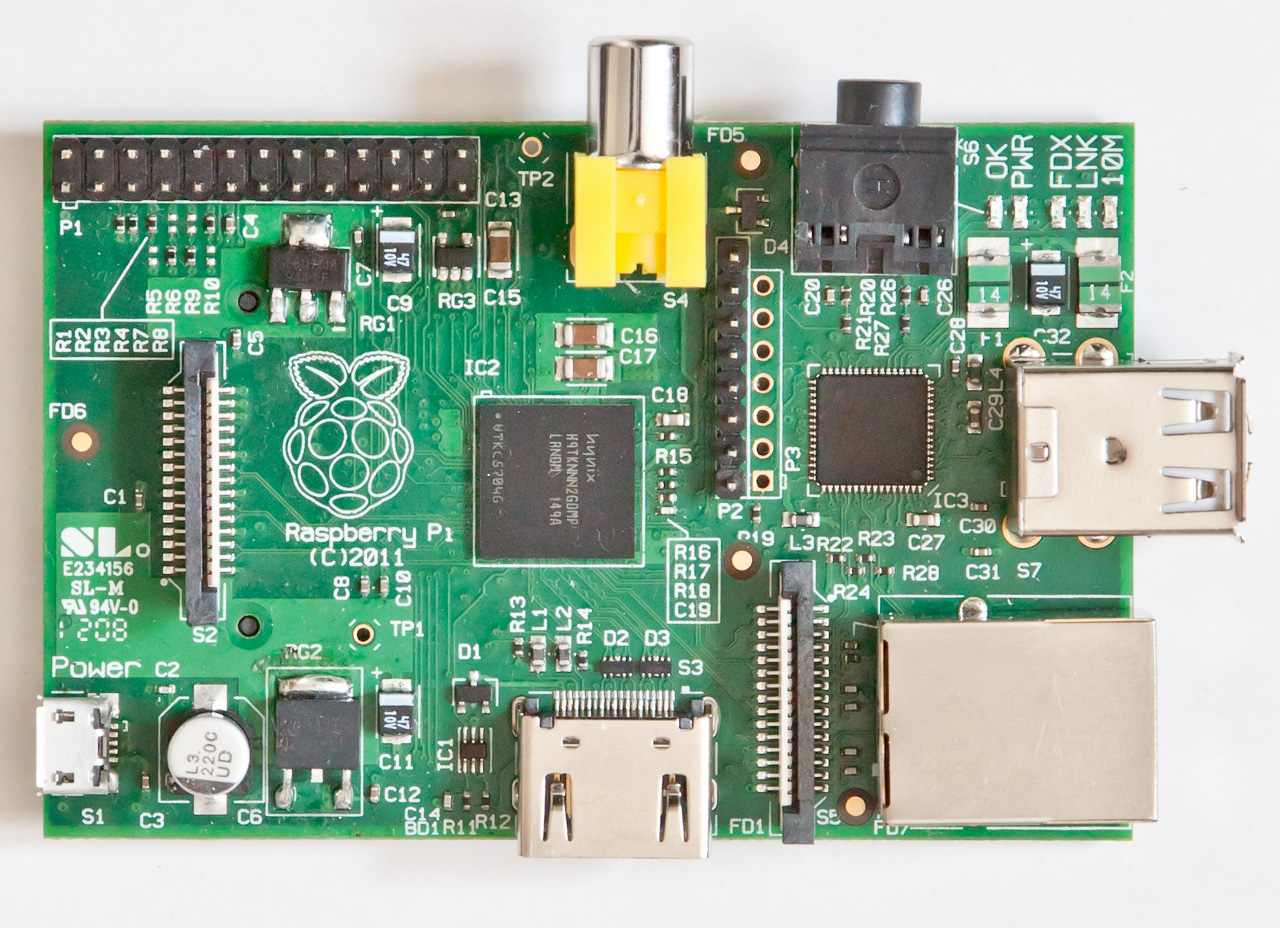
\includegraphics[width=0.55\textwidth]{./fotos/Raspberry_Pi_B_rev_1.jpg}
	\caption{RaspberryPi Model B rev1 (Quelle: \cite{rpib1})}
	\label{fig:rpib1}
\end{figure}

\begin{figure}[h!]
	\centering
		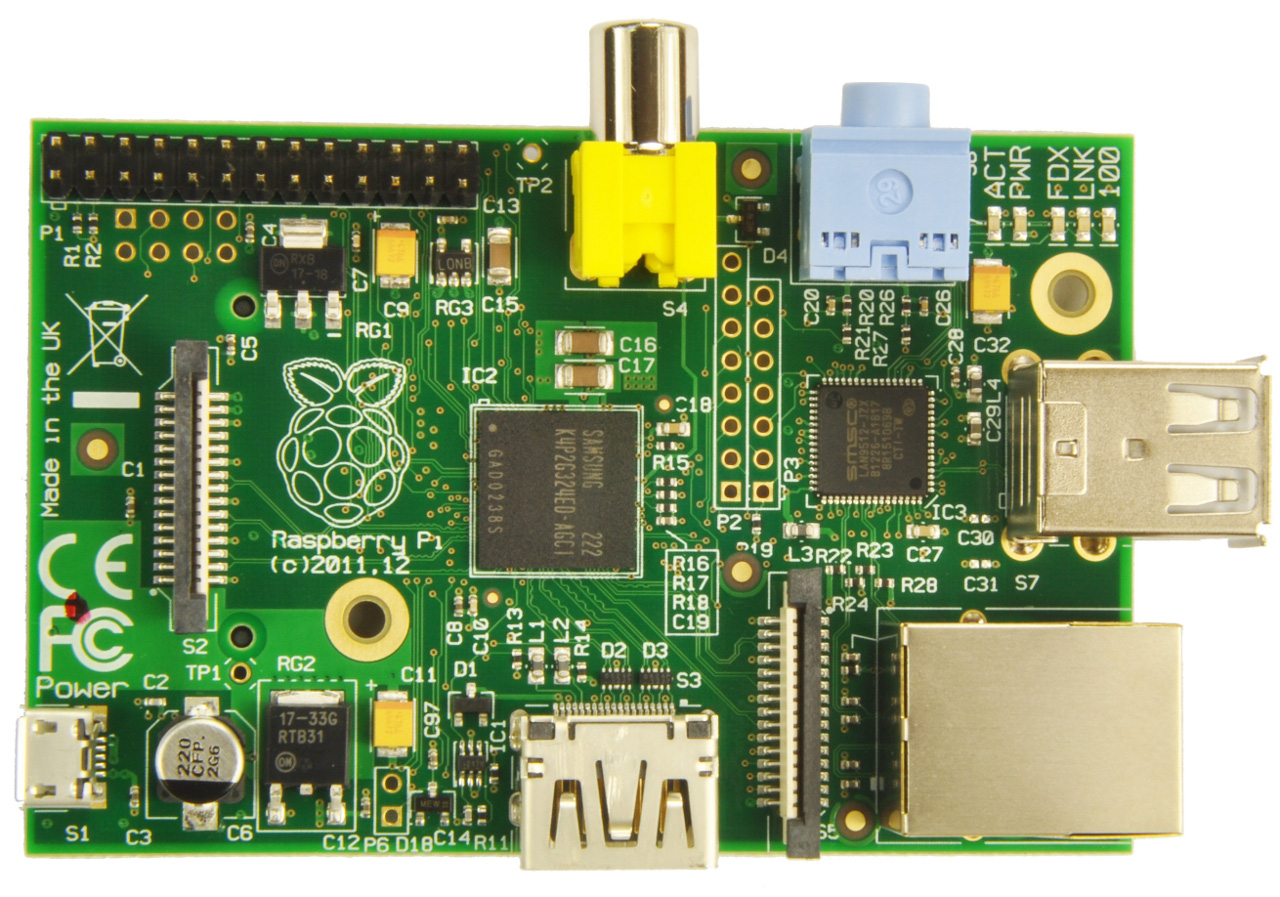
\includegraphics[width=0.55\textwidth]{./fotos/Raspberry_Pi_B_rev_2.jpg}
	\caption{RaspberryPi Model B rev2 (Quelle: \cite{rpib2})}
	\label{fig:rpib2}
\end{figure}

\begin{figure}[h!]
	\centering
		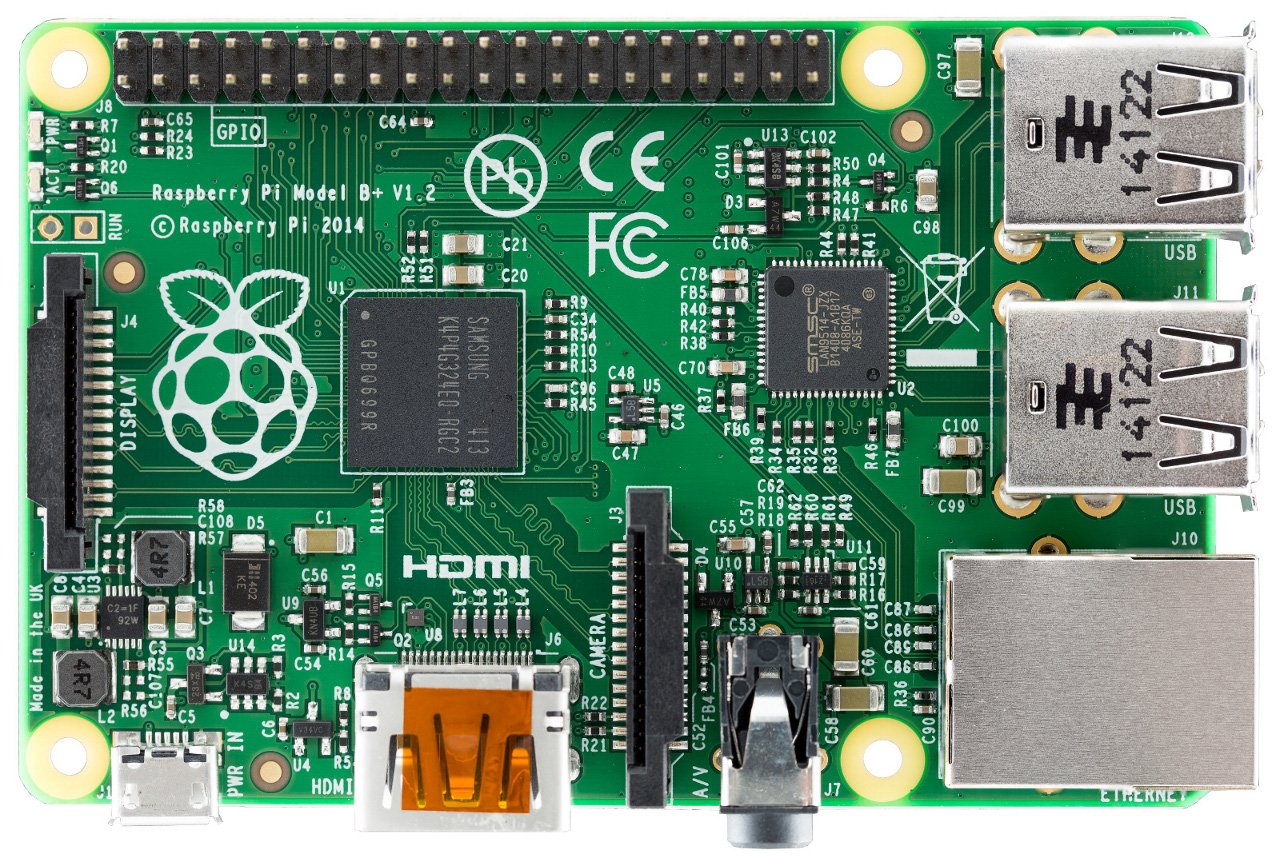
\includegraphics[width=0.55\textwidth]{./fotos/Raspberry_Pi_B+_top.jpg}
	\caption{RaspberryPi Model B+ (Quelle: \cite{rpibplus})}
	\label{fig:rpibplus}
\end{figure}

\begin{figure}[h!]
	\centering
		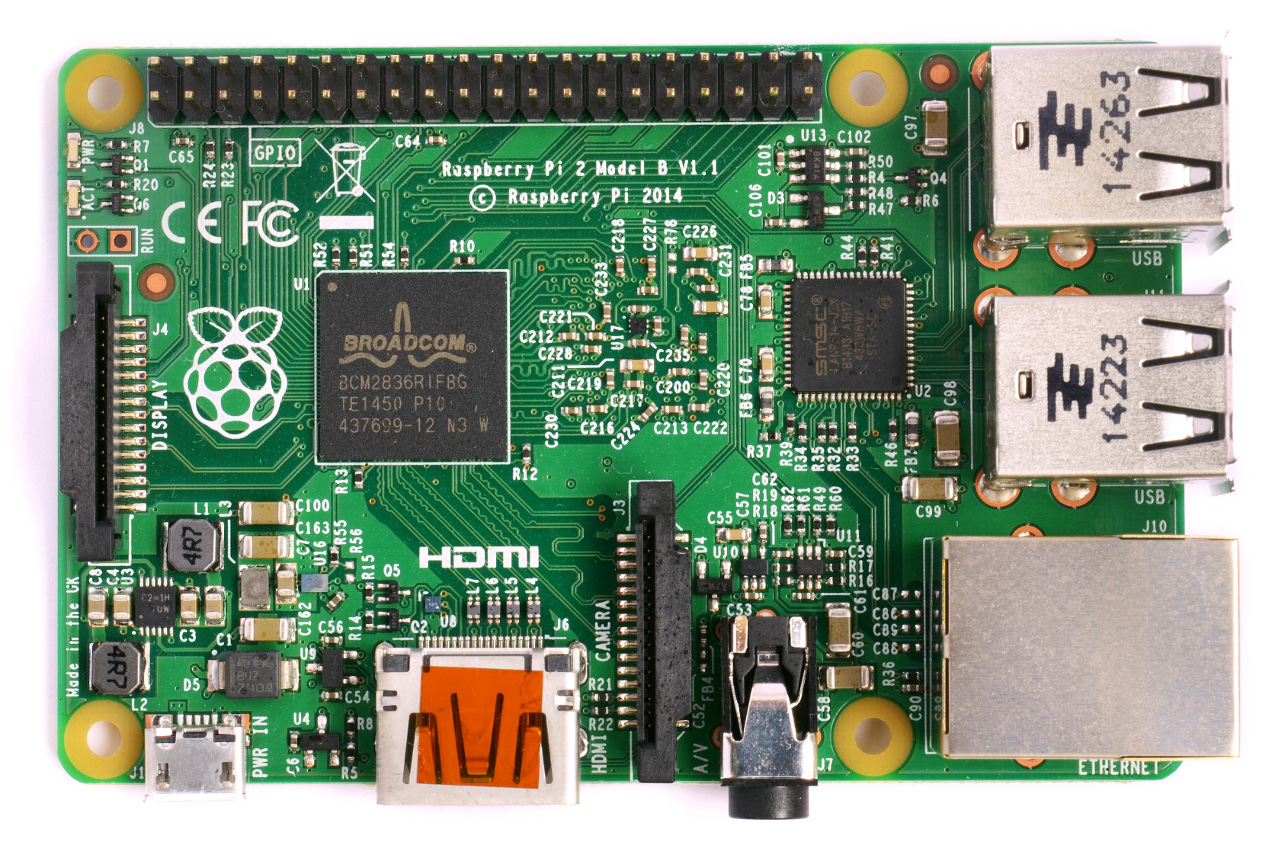
\includegraphics[width=0.55\textwidth]{./fotos/Raspberry_Pi_2_Model_B_v1-1_top_new.jpg}
	\caption{RaspberryPi 2 Model B (Quelle: \cite{rpi2b})}
	\label{fig:rpi2b}
\end{figure}

\clearpage

Auf dem RaspberryPi läuft üblicherweise eine Version von Linux (z.b. raspbian \cite{raspbian}).
Auch wer noch überhaupt keine Erfahrung mit Linux hat, kann den Infoscreen mit der Schritt-für-Schritt Anleitung (siehe \refsec{schritte}) leicht einrichten.

% \clearpage

Hier eine Auflistung von empfehlenswerten bzw. notwendigem Zubehör. Ebenso einige Links zu Preisvergleichs-Seiten bzw. Händlern und ungefähre Preise.
\begin{itemize}
	\item \textbf{RaspberryPi 2 Model B}\\
		Preis: ca. 35 Euro\\
		Beispiele für Händler:\\
		Geizhals: \url{https://geizhals.at/raspberry-pi-2-modell-b-a1225369.html}\\
		Farnell: \url{http://at.farnell.com/jsp/search/productdetail.jsp?sku=2461029}
	\item \textbf{Gehäuse} (Achtung: Gehäuse für verschiedene Modelle sind teilweise nicht kompatibel)\\
		Empfehlenswert, da das RaspberryPi ohne Gehäuse geliefert wird.\\
		Preis: ca. 10 Euro\\
		Beispiele für Händler:\\
		Farnell: \url{http://at.farnell.com/jsp/search/productdetail.jsp?sku=2426744}\\
%		e-tec.at: \url{http://www.e-tec.at/frame1/details.php?art=174576}\\
		Amazon: \url{http://www.amazon.de/dp/B00LMEEAS6}
	\item \textbf{micro SD-Karte 8GB} (Achtung: Model B benötigt eine normale SD-Karte)\\
		Notwendig zur Installation des Betriebssytems (wird oft auch günstiger als Paket verkauft).\\
		Preis: ca. 8 Euro\\
		Beispiele für Händler:\\
		Geizhals: \url{https://geizhals.at/?cat=sm_sdhc&xf=307_8~342_Class+10#xf_top}\\
		Farnell: \url{http://at.farnell.com/jsp/search/productdetail.jsp?sku=2428393}
	\item \textbf{Netzteil micro-USB 5V}\\
		Notwendig zur Stromversorgung.\\
		Preis: ca. 7 Euro\\
		Beispiele für Händler:\\
		Geizhals: \url{https://geizhals.at/raspberry-pi-netzteil-fuer-pi-type-b-765-3311-a1150197.html}\\
		Farnell: \url{http://at.farnell.com/jsp/search/productdetail.jsp?sku=2254794}
\end{itemize}

Per USB kann eine beliebige Maus und Tastatur angeschlossen werden. 
Ebenso wird ein SD- bzw. micro SD-Kartenleser zum Kopieren der Betriebsystem-Dateien benötigt. 
Zum Anschluss an die vorhandene Netzwerkinfrastruktur ist weiters ein LAN-Kabel erforderlich.


